\section{Database}\label{sec:testdatabase}
% introduktion
I det følgende vil test og integration af databasen blive beskrevet. Alle komponenter er udviklet iterativt og integreret løbende.

\subsection{UserAccess}
% klassens opgave... 
\textit{UserAccess} har til ansvar at håndtere operationer som tager \textit{User}'s ind og up af databasen. Klassen er implementeret som det første i DAL og har dannet grundlag for videre udvikling.

\subsubsection{Testdetaljer}
% beskrivelse af coverage procent og antallet af test, samt begrundelse for begge.
\textit{UserAccess.Unit.Test} har en coverage procent på 100\% og er dækket af 33 test. Med disse test er både normale brugs- og fejlscenarier dækket.

% BILLEDE AF KØRTE UNITTEST
\begin{figure}[H]
\centering
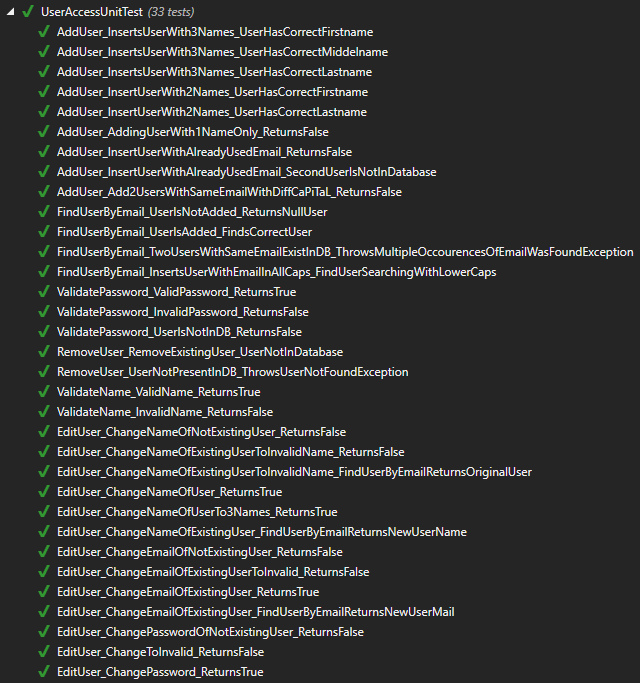
\includegraphics[width=0.9\linewidth]{figs/test/useraccessunittest}
\caption{Unittest for UserAccess.}
\label{fig:useraccessunittest}
\end{figure}

% BILLEDE AF COVERAGE KØRT
\begin{figure}[H]
\centering
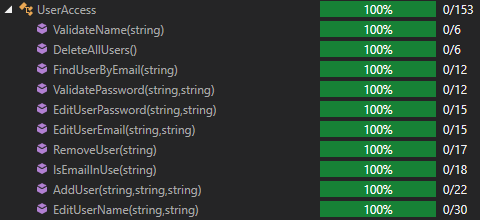
\includegraphics[width=0.7\linewidth]{figs/test/useraccesscoverage}
\caption{Coverage for UserAccess.}
\label{fig:useraccesscoverage}
\end{figure}

\subsection{Testbeskrivelse}
% hvordan div. test er valgt og hvad I specielt var opmærksom på under udviklign af test.
For hver metode er det normale brugsscenarie identificeret og testet for forskellige kombinationer. Herefter problemerne forsøgt identificeret og taget højde for.
 
% hvad var let/svært at teste etc.

\subsection{PoolAccess}
% klassens opgave... 

\subsubsection{Testdetaljer}
% beskrivelse af coverage procent og antallet af test, samt begrundelse for begge.

% BILLEDE AF KØRTE UNITTEST

% BILLEDE AF COVERAGE KØRT

\subsection{Testbeskrivelse}
% hvordan div. test er valgt og hvad I specielt var opmærksom på under udviklign af test. 
% hvad var let/svært at teste etc.

\subsection{DataAccess}
% klassens opgave... 

\subsubsection{Testdetaljer}
% beskrivelse af coverage procent og antallet af test, samt begrundelse for begge.

% BILLEDE AF KØRTE UNITTEST

% BILLEDE AF COVERAGE KØRT

\subsection{Testbeskrivelse}
% hvordan div. test er valgt og hvad I specielt var opmærksom på under udviklign af test. 
% hvad var let/svært at teste etc.